\documentclass[11pt, a4paper]{article}

\usepackage[a4paper, top=2.5cm, bottom=2.5cm, left=2cm, right=2cm]{geometry}
\usepackage{amsmath}
\usepackage{amssymb}
\usepackage{booktabs}
\usepackage{array}
\usepackage{tikz}

\title{}
\author{}
\date{}

\begin{document}

\section{Probabilistic Formulation}

\noindent \textbf{Variables.}
\begin{itemize}
    \item $x \in \mathbb{R}^D$: observation.
    \item $K$: total number of concepts in the dictionary.
    \item $d$: dimensionality of each continuous concept embedding.
    \item $c \in \{0,1\}^K$: binary concept activation mask (latent variable).
    \item $z \in \mathbb{R}^{K \times d}$: continuous concept embeddings (latent variable).
    \item $h_k \in \mathbb{R}^d$: global learnable prototypes.
    \item $\mu_k(x)$: encoder output (deterministic mean for $z_k$).
    \item $\alpha_k(x) \in [0,1]$: Bernoulli parameter representing the probability of concept activation.
\end{itemize}

\subsection{Generative Model}

We assume the latent embeddings follow a hierarchical \textbf{Gated Gaussian} prior. The binary mask $c_k$ acts as a gate: if the concept is inactive ($c_k=0$), the embedding $z_k$ is drawn from a base Gaussian distribution centered at the origin. If the concept is active ($c_k=1$), it is drawn from a shifted Gaussian distribution centered around the learnable concept prototype $h_k$. We assume a uniform prior probability $\pi$ across all concepts.

This establishes a strict generative flow ($c \to z \to x$): the discrete mask $c$ dictates the spatial location of the continuous embedding $z$, and the observation $x$ is generated from $z$.

\textbf{Priors:}
\[
p(c_k) = \operatorname{Bern}(c_k; \pi)
\]
\[
p(z_k \mid c_k) = \mathcal{N}(z_k; c_k \cdot h_k, I)
\]

\textbf{Likelihood:}
\[
p_\phi(x \mid z) = \mathcal{N}\!\bigl(x; g_\phi(z), I\bigr)
\]

\begin{figure}[htbp]
    \centering
    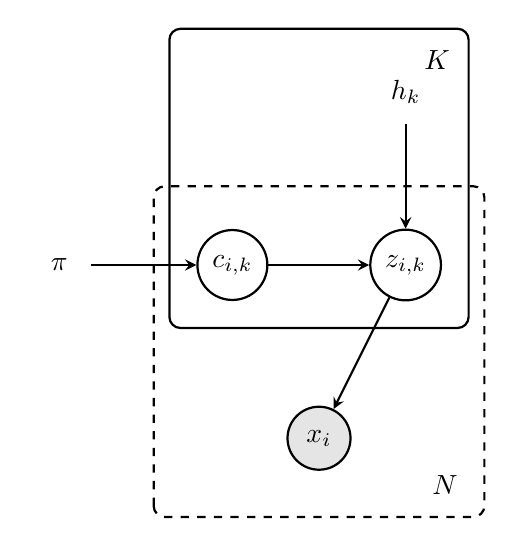
\begin{tikzpicture}[
        obs/.style={circle, draw=black, fill=gray!20, thick, minimum size=8mm},
        lat/.style={circle, draw=black, fill=white, thick, minimum size=8mm},
        param/.style={minimum size=8mm}
    ]
        % Nodes
        \node[param] (pi) at (-2.2, 0) {$\pi$};
        \node[lat] (c) at (0, 0) {$c_{i,k}$};
        \node[lat] (z) at (2.2, 0) {$z_{i,k}$};
        \node[param] (h) at (2.2, 2.2) {$h_k$};
        \node[obs] (x) at (1.1, -2.2) {$x_i$};

        % Edges
        \draw[->, >=stealth, thick] (pi) -- (c);
        \draw[->, >=stealth, thick] (h) -- (z);
        \draw[->, >=stealth, thick] (c) -- (z);
        \draw[->, >=stealth, thick] (z) -- (x);

        % Plate K (Solid)
        \draw[rounded corners, thick] (-0.8, -0.8) rectangle (3.0, 3.0);
        \node at (2.6, 2.6) {$K$};

        % Plate N (Dashed)
        \draw[rounded corners, thick, dashed] (-1.0, -3.2) rectangle (3.2, 1.0);
        \node at (2.7, -2.8) {$N$};

    \end{tikzpicture}
    \caption{Probabilistic Graphical Model of the generative process. Unshaded nodes represent latent variables, shaded nodes represent observed variables, and unboxed text represents deterministic global parameters. The solid rectangle denotes replication over $K$ concepts, while the dashed rectangle denotes replication over $N$ observations in the dataset.}
    \label{fig:pgm}
\end{figure}

\subsection{Inference Model}

Exact inference requires marginalizing over the continuous $z$ and summing over all $2^K$ possible discrete mask configurations for $c$. To maintain tractability, we employ amortized variational inference via an encoder $f_\theta(x)$ that predicts the shared parameters for the latent variables.

\textbf{Embedding Posterior:} \\
We freeze the posterior variance to a constant hyperparameter $\sigma_0^2$. The continuous embeddings are sampled using the reparameterization trick: $z_k = \mu_k(x) + \sigma_0 \cdot \epsilon$, where $\epsilon \sim \mathcal{N}(0, I)$.
\[
q_\theta(z_k \mid x) = \mathcal{N}(z_k; \mu_k(x), \sigma_0^2 I)
\]

\textbf{Dependent Mask Posterior:} \\
To accurately invert the generative flow ($x \to z \to c$), the inference model derives the Bernoulli parameter $\alpha_k(x)$ directly from the predicted spatial location $\mu_k(x)$. We compute this by evaluating the similarity between $\mu_k(x)$ and the global prototype $h_k$, scaled by a temperature $\tau$. As proven in \textbf{Appendix A.1}, this formulation is the mathematically optimal parametric form dictated by the Gated Gaussian prior.
\[
\alpha_k(x) = \operatorname{sigmoid}\!\left(\frac{\operatorname{sim}(\mu_k(x), h_k)}{\tau}\right)
\]
To enable end-to-end optimization through the discrete mask, we draw the actual latent activation $c_k$ using the continuous Gumbel-Sigmoid relaxation during training, parameterized by a Gumbel temperature $\tau_g$:
\[
c_k \sim \text{Gumbel-Sigmoid}(\alpha_k(x), \tau_g)
\]
\[
q_\theta(c_k \mid x) = \operatorname{Bern}(c_k; \alpha_k(x))
\]

\subsection{Evidence Lower Bound}

The general objective minimized over a batch of size $B$ includes an explicit per-sample entropy term $\mathcal{H}$ to enforce binarization, alongside a batch-wise sparsity KL penalty:

\[
\mathcal{L} = \frac{1}{B} \sum_{i=1}^B \left[ \mathbb{E}_{q}[\text{Recon}_i] + \gamma \sum_{k=1}^K \mathbb{E}_{q(c_{i,k})} [ D_{\mathrm{KL}}(q(z_{i,k}) \parallel p(z_{i,k} \mid c_{i,k})) ] + \lambda_{\text{ent}} \sum_{k=1}^K \mathcal{H}(\alpha_{i,k}) \right] + \beta \sum_{k=1}^K D_{\mathrm{KL}}(\bar{\alpha}_k \parallel \pi)
\]

\textit{(where $\mathcal{H}(\alpha) = -[\alpha \log(\alpha) + (1-\alpha) \log(1-\alpha)]$ is the binary entropy function).} \\
\textit{*Note on KL direction: The ELBO relies on the reverse KL divergence $D_{\mathrm{KL}}(q \parallel p)$, rather than the forward KL used in maximum likelihood estimation.}

\paragraph{Simplified Loss (Stochastic Decoding)}

\begin{equation}
    \begin{aligned}
        \mathcal{L}_{\text{simple}} &= \frac{1}{B} \sum_{i=1}^B \left[ \|x_i - \hat{x}_i\|^2
        + \gamma \sum_{k=1}^K \left( \text{sg}(\alpha_{i,k}) \|\mu_{i,k} - h_k\|^2 + (1 - \text{sg}(\alpha_{i,k})) \|\mu_{i,k}\|^2 \right)
        + \lambda_{\text{ent}} \sum_{k=1}^K \mathcal{H}(\alpha_{i,k}) \right] \\
        &+ \beta \sum_{k=1}^K D_{\mathrm{KL}}(\bar{\alpha}_k \parallel \pi)
    \end{aligned}
\end{equation}

\noindent \textit{where $\hat{x}_i = g_\phi(c_i \odot z_i)$ is the stochastic reconstruction.}

\vspace{0.3cm}
\noindent \textit{Derivation Details:}
\begin{itemize}
    \item \textbf{Variance Constant:} Because the posterior variance $\sigma_0^2$ is fixed, the variance penalty terms in the standard Gaussian KL divergence become static constants and drop out of the optimization objective. The Conditional KL simplifies to a pure squared $L_2$ distance on the expected locations.
    \item \textbf{Magnitude Penalty:} We pass the \textbf{unnormalized} embedding $z_{i,k}$ to the decoder. To prevent the encoder from scaling up $\|\mu_{i,k}\|$ to push signal through a closed mask, we apply $(1 - \text{sg}(\alpha_{i,k})) \|\mu_{i,k}\|^2$ as a dynamic weight decay on inactive concepts.
    \item \textbf{Stop-Gradient:} The $\text{sg}(\cdot)$ operator (\texttt{.detach()}) prevents the network from artificially driving $\alpha_{i,k} \to 0$ solely to minimize the $\gamma$ structural penalty.
\end{itemize}

\subsection{Similarity Metrics}

We formulate the mask probability $\alpha_k$ using variants of the generalized $\operatorname{sim}(\cdot)$ function. Since we decode with unnormalized vectors, these metric choices dictate whether the gating mechanism is algebraically coupled to the embedding magnitude.

\begin{table}[h]
\centering
\renewcommand{\arraystretch}{1.5}
\begin{tabular}{>{\bfseries}l c c p{6cm}}
\toprule
Metric & Formulation ($L_k$) & Role of $\tau$ & Properties \\
\midrule
Cosine Similarity & $\frac{1}{\tau} \frac{\mu_k \cdot h_k}{\Vert \mu_k \Vert \Vert h_k \Vert}$ & \textbf{Mandatory} & Bounded. Angle solely controls the discrete gate, while magnitude provides expressivity to the continuous decoder. \\
Inner Product & $\frac{\mu_k \cdot h_k}{\tau}$ & \textbf{Redundant} & Unbounded. Entangles gating directly with continuous expressivity; network can artificially scale $\Vert \mu_k \Vert$. \\
Neg. Euclidean & $\frac{b - \Vert \mu_k - h_k \Vert}{\tau}$ & \textbf{Structural} & Direct geometric fit for the Gaussian prior. Requires learning the radius bias $b$. \\
\bottomrule
\end{tabular}
\end{table}

\subsection{Implementation Details}

\paragraph{Architecture}
A standard backbone (e.g., ResNet, ViT) extracts dense visual features, followed by $K$ distinct linear layers to produce the continuous means $\mu_1, \dots, \mu_K$.

\paragraph{Stochastic Gating}
We explicitly pass the masked, stochastic tensor $c \odot z$ (where $z = \mu + \sigma_0 \epsilon$) to the decoder. This guarantees inactive concepts transmit a clean zero signal, while active concepts transmit the continuous stochastic distribution to properly capture uncertainty.

\paragraph{Batch Sparsity}
The global sparsity penalty is evaluated over the batch: $D_{\mathrm{KL}}(\bar{\alpha}_k \parallel \pi)$, where $\bar{\alpha}_k = \frac{1}{B} \sum_{i=1}^B \alpha_k(x_i)$.

\paragraph{Prototype Maintenance}
We do not $L_2$-normalize $h_k$ after optimization steps. Because the active penalty is $\|\mu_{i,k} - h_k\|^2$, allowing the optimizer to freely scale $h_k$ ensures the decoder has access to dynamically sized magnitudes.

\paragraph{Binarization Pressure}
The batch-wise KL divergence lacks a per-sample force to push individual probabilities toward strict bounds. We incorporate a per-sample entropy minimization penalty $\mathcal{H}$ to prevent the model from settling on ambiguous probabilities ($\alpha_{i,k} \approx 0.5$).

\subsection{Latent Representation Topologies}

The model can be instantiated in two mathematically distinct topologies depending on how the active concept embeddings $c_k z_k$ are passed to the downstream decoder $g_\phi$.

\paragraph{1. Summed Representation ($\sum_{k} c_k z_k \in \mathbb{R}^d$)}
In this topology, the decoder receives a dense, aggregated vector. The model algebraically behaves as a \textbf{Factorial Mixture Model}.
\begin{itemize}
    \item \textbf{Superposition:} Concepts share a single coordinate system. The decoder processes a linear superposition of features.
    \item \textbf{Capacity \& Interference:} Representational capacity scales combinatorially ($2^K$ states). However, summing introduces the geometric risk of destructive interference. To utilize this topology effectively, the decoder must be capable of algebraically un-mixing overlapping prototypes.
\end{itemize}

\paragraph{2. Stacked Representation ($[c_1 z_1, \dots, c_K z_K] \in \mathbb{R}^{K \times d}$)}
In this topology, the active concepts are stacked into a sequence or structured matrix.
\begin{itemize}
    \item \textbf{Semantic Isolation:} The concepts are placed into strictly isolated semantic slots. The decoder processes each concept via independent parameter channels.
    \item \textbf{Architectural Orthogonality:} Because the concepts do not share the same algebraic coordinate space, there is zero risk of destructive interference. This topology effectively acts as $K$ parallel, fully disentangled 2-component mixture models.
\end{itemize}

\subsection{Decoder Identifiability}

To ensure that distinct latent slots map to independent visual features and to guarantee generative identifiability, we apply an explicit structural prior to the decoder's weights.

Assuming a strictly \textbf{linear decoder} (or analyzing the first hidden mixing layer of an MLP), the stacked latent tensor $Z = [c_1 z_1, \dots, c_K z_K]$ is projected via a weight matrix $W$. We partition this matrix into $K$ independent blocks $W = [W_1, W_2, \dots, W_K]$, where each block $W_k$ acts as the explicitly defined visual basis for Concept $k$:
\[
\hat{x} = \sum_{k=1}^K W_k (c_k z_k)
\]
To prevent redundant bases and enforce functional diversity across the dictionary, we introduce a Frobenius orthogonality penalty between these weight blocks:
\[
\mathcal{L}_{\text{dec\_ortho}} = \lambda_{\text{ortho}} \sum_{i \neq j} \frac{\| W_i^T W_j \|_F^2}{\|W_i\|_F^2 \|W_j\|_F^2}
\]
From a Bayesian perspective, this penalty corresponds to Maximum A Posteriori (MAP) estimation under a structural prior $p(\phi)$ that heavily favors orthogonal basis weights. Mathematically forbidding $W_i$ and $W_j$ from mapping to the same downstream features fundamentally prevents capacity cannibalization. Once the network is restricted from using redundant slots to reconstruct high-frequency modes, the optimizer naturally allocates freed slots to span the remaining unexplained variance in the dataset.

\subsection{Related Work}

Our probabilistic formulation conceptually bridges several established paradigms in representation learning, structurally formalizing the relationships between discrete routing and continuous generation.

\paragraph{Concept Embedding Models (CEMs)}
While standard Variational Autoencoders (VAEs) utilize a dense, highly entangled continuous latent space, our framework establishes a structured bottleneck. It shares lineage with CEMs, which attach high-dimensional continuous embeddings to discrete semantic concepts. However, whereas CEMs traditionally rely on supervised concept labels to regularize these embeddings, our Gated Gaussian framework operates entirely probabilistically, supporting unsupervised or weakly-supervised concept discovery via the evidence lower bound (ELBO).

\paragraph{Vector-Quantized Autoencoders (VQ-VAEs)}
Our framework provides a probabilistic counterpart to discrete quantization models like VQ-VAEs, but with inverted routing mechanisms. A VQ-VAE routes categorical (one-hot) decisions into \textit{spatial} slots using rigid codebook vectors, limiting the representational capacity of a single bottleneck to $K$ discrete states. In contrast, our framework routes independent Bernoulli probabilities into isolated \textit{semantic} slots using gated continuous distributions. This preserves the high-fidelity expressivity and uncertainty handling of continuous VAEs while achieving the interpretable routing of discrete bottlenecks.

\paragraph{Basis Decomposition and Semantic Embeddings}
Models such as Interpretable Basis Decomposition (IBD) and Knowledge Graph (KG) Embeddings project features into a shared, dense coordinate space where representations are formed via algebraic combinations. In these shared spaces, concepts risk destructive interference (polysemy entanglement) and typically require heavy geometric regularization. Our \textit{Stacked} topology naturally circumvents this entanglement by treating concepts as parallel, structurally orthogonal mixture models, explicitly avoiding the un-mixing problem inherent to linearly summed latent spaces.

\appendix
\section{Mathematical Derivations}

\subsection{Optimal Gating Mechanism (Derivation of $\alpha$)}
To mathematically justify the similarity-based gating, we can derive the optimal form of the mask posterior directly from the generative priors using Bayes' rule. We express the true posterior probability of a concept being active given its embedding as a log-odds ratio:

\[
\log \frac{p(c_k = 1 \mid z_k)}{p(c_k = 0 \mid z_k)} = \log \frac{p(z_k \mid c_k = 1) p(c_k = 1)}{p(z_k \mid c_k = 0) p(c_k = 0)}
\]

Substituting the Gated Gaussian priors ($\mathcal{N}(h_k, I)$ for the active state, $\mathcal{N}(0, I)$ for the inactive state) and canceling shared normalizing constants yields:

\[
\text{Log-Odds} = -\frac{1}{2}\|z_k - h_k\|^2 + \frac{1}{2}\|z_k\|^2 + \operatorname{logit}(\pi)
\]

By algebraically expanding the squared distance ($\|z_k - h_k\|^2 = \|z_k\|^2 - 2 z_k^T h_k + \|h_k\|^2$), the $\frac{1}{2}\|z_k\|^2$ terms perfectly cancel out:

\[
\text{Log-Odds} = z_k^T h_k - \frac{1}{2}\|h_k\|^2 + \operatorname{logit}(\pi)
\]

Converting the log-odds back to a probability via the sigmoid function, and substituting the encoder's predicted mean $\mu_k$ for $z_k$, we recover an exact inner-product formulation:

\[
\alpha_k \approx \operatorname{sigmoid}\left( \mu_k^T h_k - \text{Bias}_k \right)
\]

This proves that tying a concept's probability of being active ($\alpha_k$) to its spatial proximity to its prototype ($h_k$) is not an arbitrary heuristic, but the optimal parametric form dictated by the Gated Gaussian prior.

\subsection{Explicit ELBO Derivation}

To maximize the log marginal likelihood of the data $\log p(x)$, we introduce the approximate posterior $q(c, z \mid x)$ and apply Jensen's Inequality to derive the Evidence Lower Bound (ELBO).

\textbf{Step 1: The Lower Bound}\\
To compute the log marginal likelihood of the data $\log p(x)$, we must marginalize over all possible latent states. Because this integral over the continuous $z$ and sum over the discrete $c$ is computationally intractable, we introduce our approximate posterior $q(c, z \mid x)$ and multiply the integrand by $1 = \frac{q(c, z \mid x)}{q(c, z \mid x)}$:

\[
\log p(x) = \log \sum_c \int p(x, c, z) \frac{q(c, z \mid x)}{q(c, z \mid x)} \, dz
\]

This allows us to mathematically rewrite the expression as an expectation over our approximate posterior:

\[
\log p(x) = \log \left( \mathbb{E}_{q(c, z \mid x)}\left[ \frac{p(x, c, z)}{q(c, z \mid x)} \right] \right)
\]

Because the logarithm is a concave function, we can apply \textbf{Jensen's Inequality} ($\log \mathbb{E}[Y] \ge \mathbb{E}[\log Y]$) to move the logarithm inside the expectation. This bounds the log-likelihood from below, giving us the Evidence Lower Bound (ELBO) that we can maximize:

\[
\log p(x) \ge \mathbb{E}_{q(c, z \mid x)}\left[\log \frac{p(x, c, z)}{q(c, z \mid x)}\right] \equiv \text{ELBO}
\]

\textbf{Step 2: Factorizing the Distributions}\\
Based on our hierarchical generative model, the joint distribution factorizes over the independent concepts as:

\[
p(x, c, z) = p(x \mid z) \prod_{k=1}^K p(c_k) p(z_k \mid c_k)
\]

Because the encoder outputs shared deterministic parameters $\mu(x)$ from which both $c$ and $z$ distributions are independently sampled, the approximate posterior factorizes exactly:

\[
q(c, z \mid x) = \prod_{k=1}^K q(c_k \mid x) q(z_k \mid x)
\]

\textbf{Step 3: Expanding the Expectation}\\
First, we substitute the factorized distributions directly into the ELBO fraction:

\[
\text{ELBO} = \mathbb{E}_{q(c, z \mid x)} \left[ \log \frac{p(x \mid z) \prod_{k=1}^K p(c_k) p(z_k \mid c_k)}{\prod_{k=1}^K q(c_k \mid x) q(z_k \mid x)} \right]
\]

Because the products in the numerator and denominator share the same index $k$, we can group the terms inside a single product block:

\[
\text{ELBO} = \mathbb{E}_{q(c, z \mid x)} \left[ \log \left( p(x \mid z) \prod_{k=1}^K \frac{p(c_k)}{q(c_k \mid x)} \frac{p(z_k \mid c_k)}{q(z_k \mid x)} \right) \right]
\]

Next, using the properties of logarithms ($\log(A \cdot B) = \log A + \log B$ and $\log \prod A_k = \sum \log A_k$), the logarithm converts the multiplication into addition and the product into a sum, cleanly separating the likelihood from the concept distributions:

\[
\text{ELBO} = \mathbb{E}_{q(c, z \mid x)} \left[ \log p(x \mid z) + \sum_{k=1}^K \log \frac{p(c_k)}{q(c_k \mid x)} + \sum_{k=1}^K \log \frac{p(z_k \mid c_k)}{q(z_k \mid x)} \right]
\]

\textbf{Step 4: Grouping into KL Divergences}\\
By linearity of expectation and the definition of Kullback-Leibler divergence, we can cleanly separate this equation into three core components:

\begin{enumerate}
    \item \textbf{Reconstruction Term:}
    \[
    \mathbb{E}_{q(c, z \mid x)}[\log p(x \mid z)]
    \]

    \item \textbf{Mask Prior KL:}
    \[
    \sum_{k=1}^K \mathbb{E}_{q(c_k \mid x)} \left[ \log \frac{p(c_k)}{q(c_k \mid x)} \right] = - \sum_{k=1}^K D_{\mathrm{KL}}(q(c_k \mid x) \parallel p(c_k))
    \]

    \item \textbf{Conditional Embedding KL:}\\
    Because the expected distribution of $z_k$ depends on the activation of $c_k$ in the prior, the expectation for the $z$ embeddings must be taken over the predicted distribution of $c$:
    \[
    \sum_{k=1}^K \mathbb{E}_{q(c_k \mid x)} \left[ \mathbb{E}_{q(z_k \mid x)} \left[ \log \frac{p(z_k \mid c_k)}{q(z_k \mid x)} \right] \right] = - \sum_{k=1}^K \mathbb{E}_{q(c_k \mid x)} \left[ D_{\mathrm{KL}}(q(z_k \mid x) \parallel p(z_k \mid c_k)) \right]
    \]
\end{enumerate}

\textbf{Step 5: The Final Analytical ELBO}\\
Combining the terms, the mathematically pure Evidence Lower Bound to maximize is:

\[
\text{ELBO} = \underbrace{\mathbb{E}_{q}[\log p(x \mid z)]}_{\text{Reconstruction}} - \underbrace{\sum_{k=1}^K D_{\mathrm{KL}}(q(c_k \mid x) \parallel p(c_k))}_{\text{Sparsity}} - \underbrace{\sum_{k=1}^K \mathbb{E}_{q(c_k \mid x)} \left[ D_{\mathrm{KL}}(q(z_k \mid x) \parallel p(z_k \mid c_k)) \right]}_{\text{Conditional Embedding}}
\]

\vspace{0.5cm}
\noindent \textbf{Connection to Our Practical Loss Objective ($\mathcal{L}$):}\\
To minimize this as a deep learning loss, we negate the ELBO. In our practical formulation, we retain the \textbf{Reconstruction} and \textbf{Conditional Embedding KL} terms derived above (substituting the empirical decoding structure $c \odot z$). To prevent "dead concepts" across the dataset, we replace the analytical per-sample \textit{Mask Prior KL} with a global, batch-wise sparsity penalty $\beta \sum_k D_{\mathrm{KL}}(\bar{\alpha}_k \parallel \pi)$. Because swapping to a batch-wise mean strips away the natural per-sample binarization pressure found in the discrete KL formula, we explicitly inject the missing entropy component back into the objective as our $\lambda_{\text{ent}} \mathcal{H}(\alpha_{i,k})$ penalty.

\end{document}